\documentclass[10pt]{beamer}
\usepackage[utf8]{inputenc}
\usepackage[english]{babel}
\usepackage{tikz}

\newcommand{\im}{\mathrm{im}}
\newcommand{\Z}{\mathbb{Z}}
\newcommand{\R}{\mathbb{R}}

\begin{document}
\begin{frame}{Local to global}
	\begin{block}{Statement}
		Let $Y \subseteq X$ be a pair of compact Hausdorff spaces such that for any $p \in Y$ and any open neighborhood $V$ of $p$ in $X$ there exists an open neighborhood $U \subset V$ of $p$ such that $\im \big(\widetilde H_\bullet(U \cap Y) \to \widetilde H_\bullet(V)\big) = 0$. Then, $\im \big(H_d(Y) \to H_d(X)\big)$ is finitely generated for every $d$.
	\end{block}
	\pause
	\begin{block}{Counterexample}
		Take $X = Y = $ suspension of $\left\{\left(0, 2^{-n}\right)\ |\ n \geq 0\right\} \cup \{(0, 0)\} \subset \R^2$.
		\vspace*{.3cm}
		
		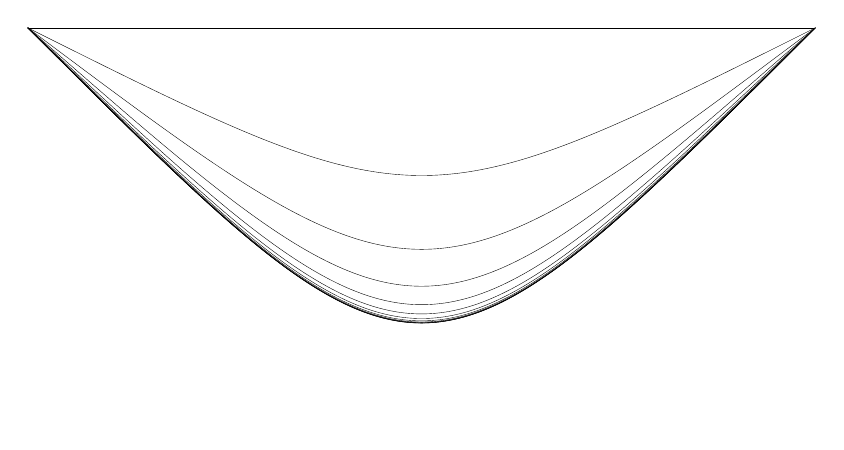
\begin{tikzpicture}[scale=5]
		\foreach \i in {0,1,2,...,12}{
			\draw[line width=0.05mm] (-1,1) .. controls (0,1/2^\i) .. (1,1);
		}
		\end{tikzpicture}
	\end{block}
	\vspace*{-1cm}
\end{frame}
\end{document}
